\documentclass{ctexart}
\usepackage{enumerate}
\usepackage[top=1in, bottom=1in, left=1.25in, right=1.25in]{geometry}
\usepackage{graphicx}
\usepackage{listings}

\author{REMOVED<REMOVED>\\学号:REMOVED}
\title{微机原理实验3\\学习使用STM32定时器}
\begin{document}

\begin{titlepage}
\maketitle
\thispagestyle{empty}
\newpage
\tableofcontents
\thispagestyle{empty}
\end{titlepage}

\setcounter{page}{1}
\lstset{language=C, 
		numbers=left, 
		frame=single,
		breaklines=true,
		breakautoindent=false,
		numberstyle=\tiny,
		fontadjust,
		basicstyle=\footnotesize
		}

\section{题目简介} 

本次实验要求学习STM32的基本定时器(TIM6和TIM7)、通用定时器(TIM2$\sim$TIM5)、高级定时器(TIM1和TIM8)以及系统时钟(“SysTick”)这四种中断源的用法,并自行编写中断处理程序,实现LED定时闪烁。

\section{题目分析}

这个题目涉及到的技术细节有:
\begin{enumerate}[1.]
\item STM32片内时钟分布
\item GPIO端口输出配置
\item 中断控制器配置
\item 三种定时器的使用
\item SysTick的重定义
\end{enumerate}
下面对这几个要点分别进行说明

\subsection{STM32片内时钟分布}

STM32片内时钟布置图比较复杂,如图\ref{stm32clocktree}所示。本次实验中,CMSIS子系统配置为默认配置,这种情况下会将8MHz的内部时钟做调整后,从内部时钟线送到锁相环,通过PLL升至72MHz作为SYSCLK。之后,通过对APB1和APB2两条外设时钟线的使能位进行配置,启用对应片上外设的时钟,即可使其工作。这个操作过程,正好体现了“时钟驱动型芯片”的概念。
\begin{figure}[!p]\centering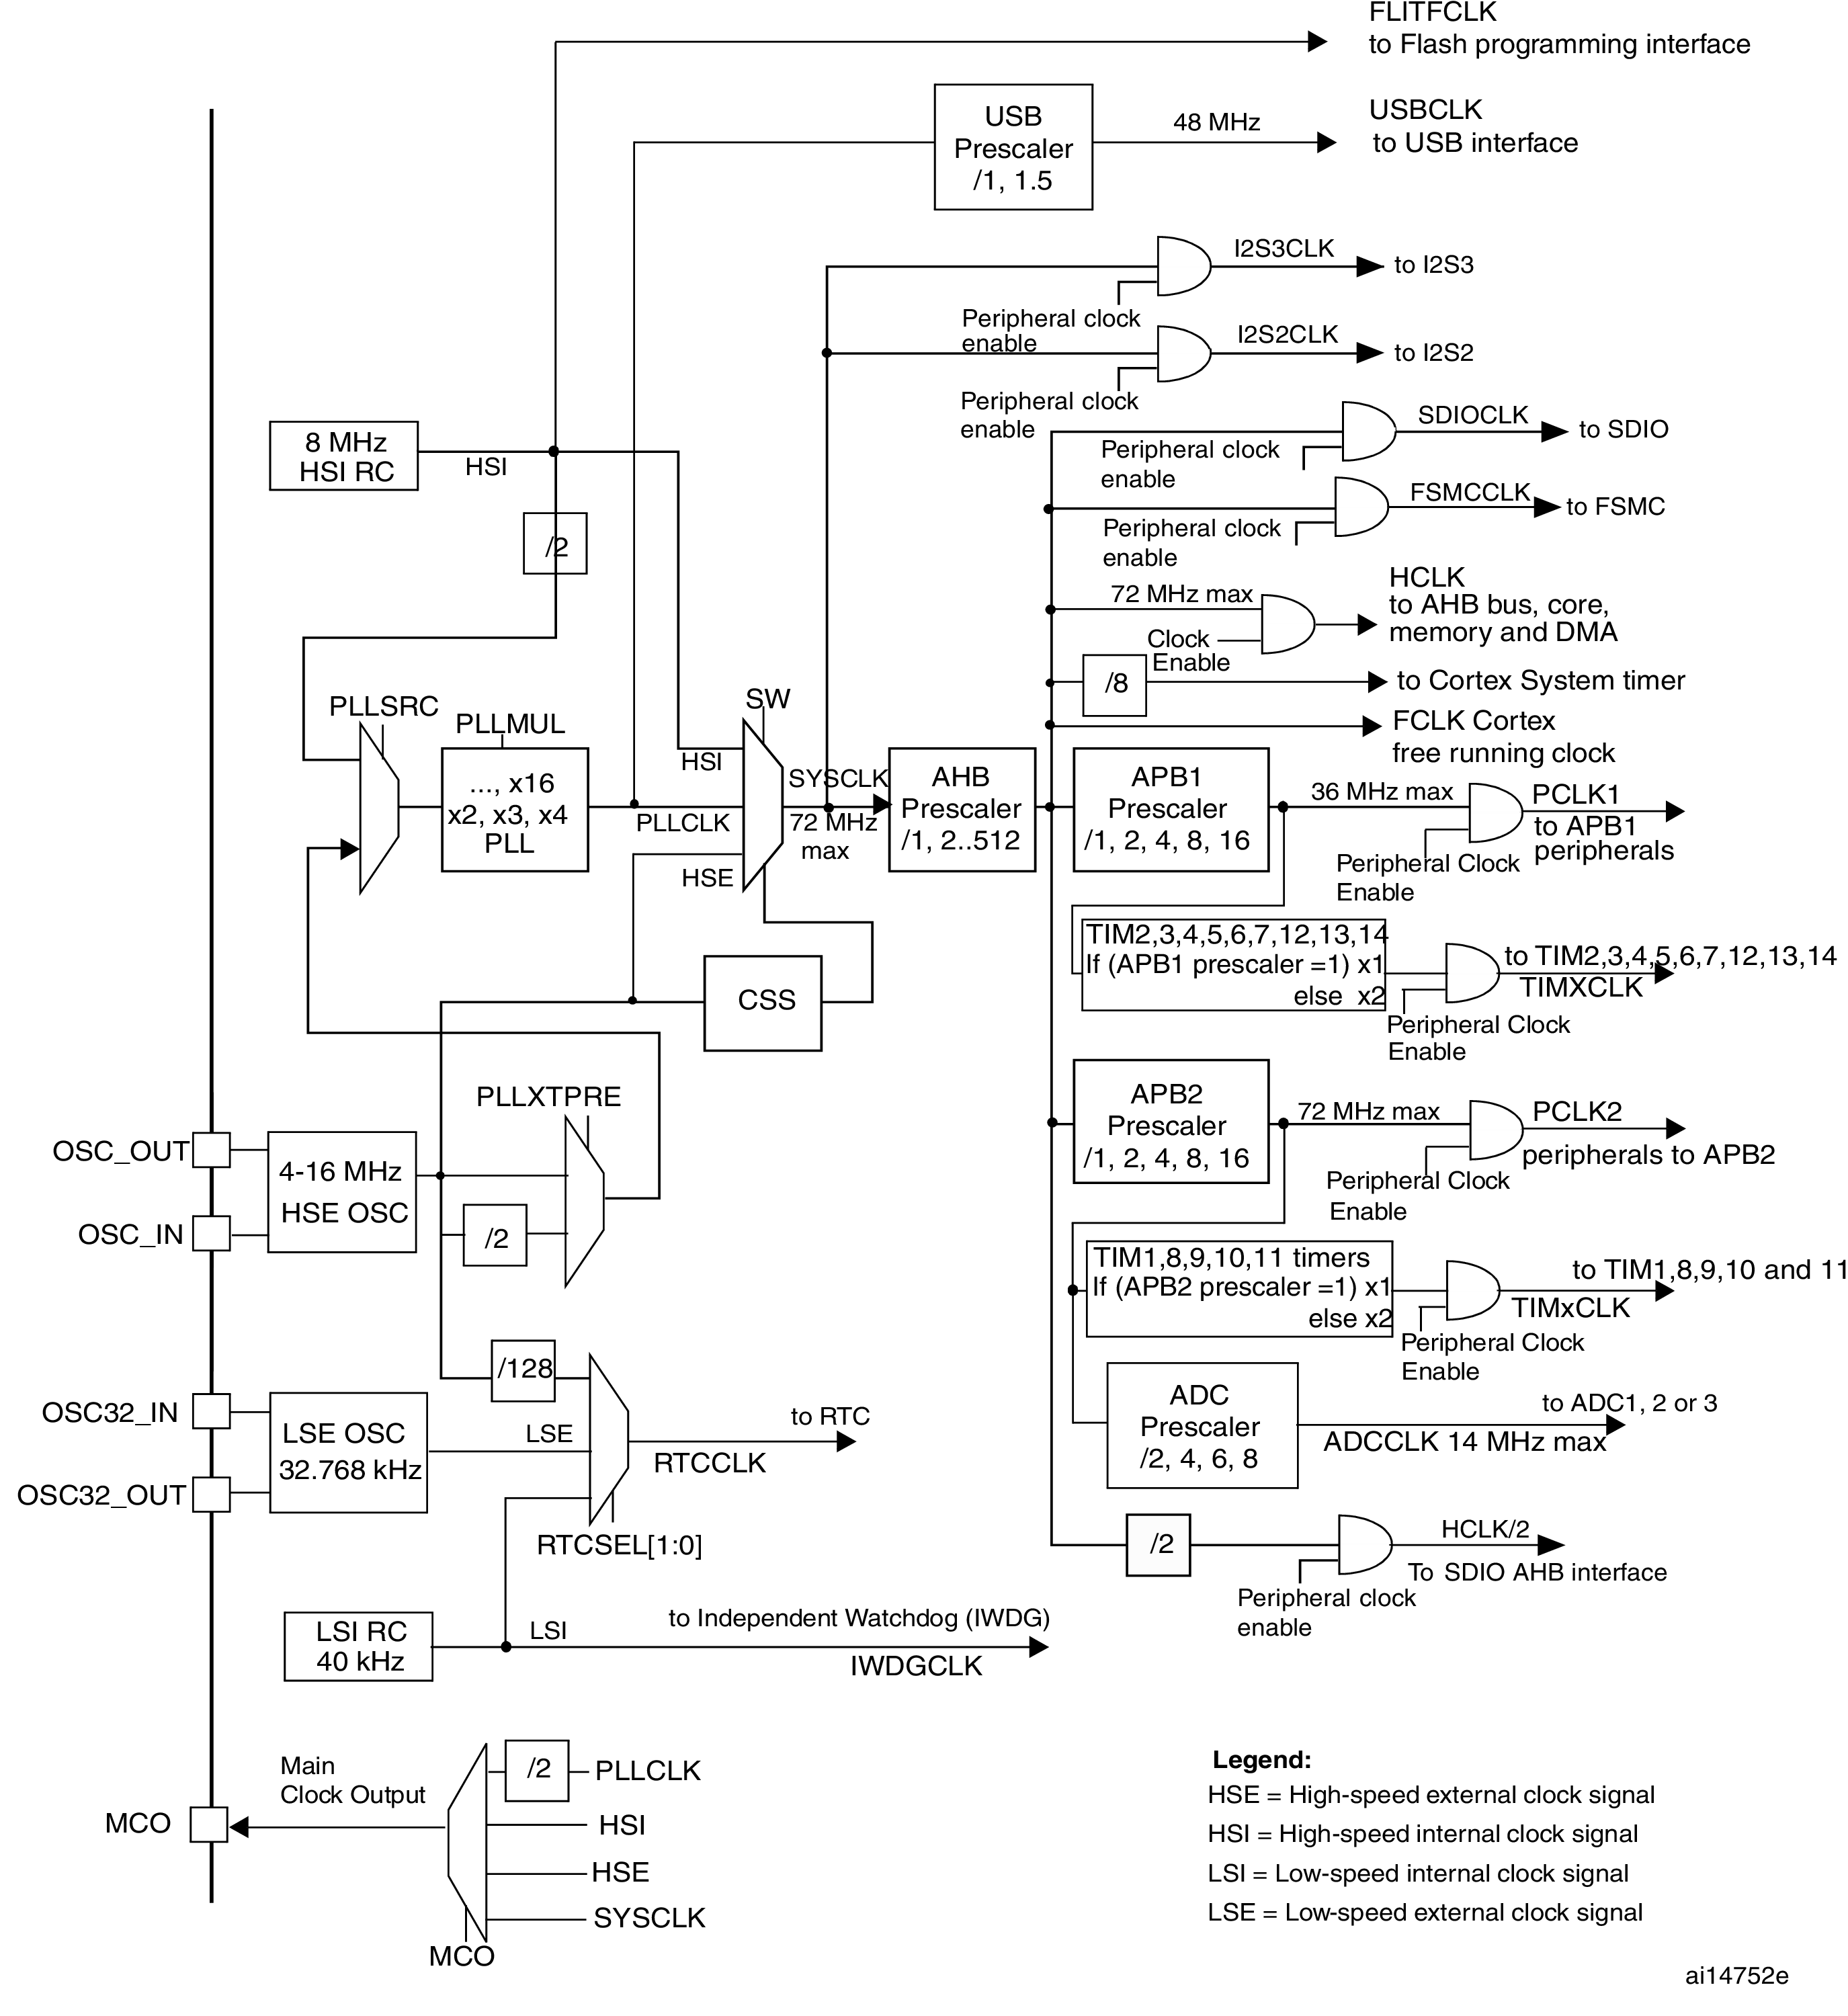
\includegraphics[width=\textwidth]{./img/clocktree.png}\caption{STM32 Clock tree}\label{stm32clocktree}\end{figure}

对时钟源的配置,是通过\lstinline{RCC_CR}的\lstinline{HSITRIM}位实现的,PLL配置则通过对\lstinline{RCC_CR}和\lstinline{RCC_CFGR}进行置位来实现。对有关APB总线下外设的时钟开关,则通过修改\lstinline{RCC_APB1ENR}和\lstinline{RCC_APB2ENR}来控制。如果直接操作寄存器,需要自行考虑片内延迟以及稳定性问题,因此在CMSIS子系统中,提供了函数\lstinline{RCC_APBxPeriphClockCmd()},可以通过该函数直接配置外设时钟开关。

进行任何操作之前要注意的是,由于STM32的这一特性,所有片上外设在使用之前,都要再三检查是否配置好了正确的时钟参数,否则可能会出现难以排查的问题。此外,通过调用\lstinline{RCC_APBxPeriphClockCmd()}对片上外设的时钟开关进行控制,可以在必要的时候关闭部分设备的电源,从而降低耗电或人为关闭部分功能。

对时钟源的误差控制,以及外部时钟源的切换,与本次实验无关,因此不做介绍。
%convert -density 500 -crop 2750x3000+870+750 'chip manual.pdf[91]' clocktree.png && gwenview clocktree.jpg

\subsection{GPIO端口输出配置}

在STM32上的架构中,GPIO端口被定义为片上外设,与其他的片上资源相同,因此在CMSIS中使用的时候,也要按照对片上外设的标准调用步骤来。他们分别是:
\begin{enumerate}
\item 用\lstinline{RCC_APBxPeriphClockCmd()}启用时钟
\item 如有必要,用\lstinline{XXX_DeInit()}清空配置。这个步骤在大型程序中比较常见,可清理上次使用片上设备时的数据。
\item 用\lstinline{XXXX_Init()}初始化配置
\item 用外设对应的函数与其交互
\end{enumerate}
GPIO是通用的输入输出端口,CMSIS中负责GPIO初始化的结构体是\lstinline{GPIO_InitTypeDef}。其原型如代码\ref{gpioperp}所示:
\begin{lstlisting}[caption={GPIOInitTypeDef},label={gpioperp}]
typedef struct
{
  uint16_t GPIO_Pin;             /*!< Specifies the GPIO pins to be configured.*/
  GPIOSpeed_TypeDef GPIO_Speed;  /*!< Specifies the speed for the selected pins.*/
  GPIOMode_TypeDef GPIO_Mode;    /*!< Specifies the operating mode for the selected pins.*/
}GPIO_InitTypeDef;
\end{lstlisting}
\lstinline{GPIO_PIN}成员是用来选择待配置的接口的,\lstinline{GPIO_Speed}用来选择对应的时钟频率,这里我们选择50MHz,而最后一个\lstinline{GPIO_Mode}则是用来选择端口对应的驱动模式。这一驱动模式对应下图\ref{stm32iodriver}中的内部电路图。由于我们的LED灯正极通过1k的电阻接到电源正极,负极接入IO引脚,可以直接选择推挽输出方式,即\lstinline{GPIO_Mode_Out_PP}。关于引脚工作模式选择的具体知识,可以参考有关的模拟电路书籍,这里不再赘述。
\begin{figure}[h]\centering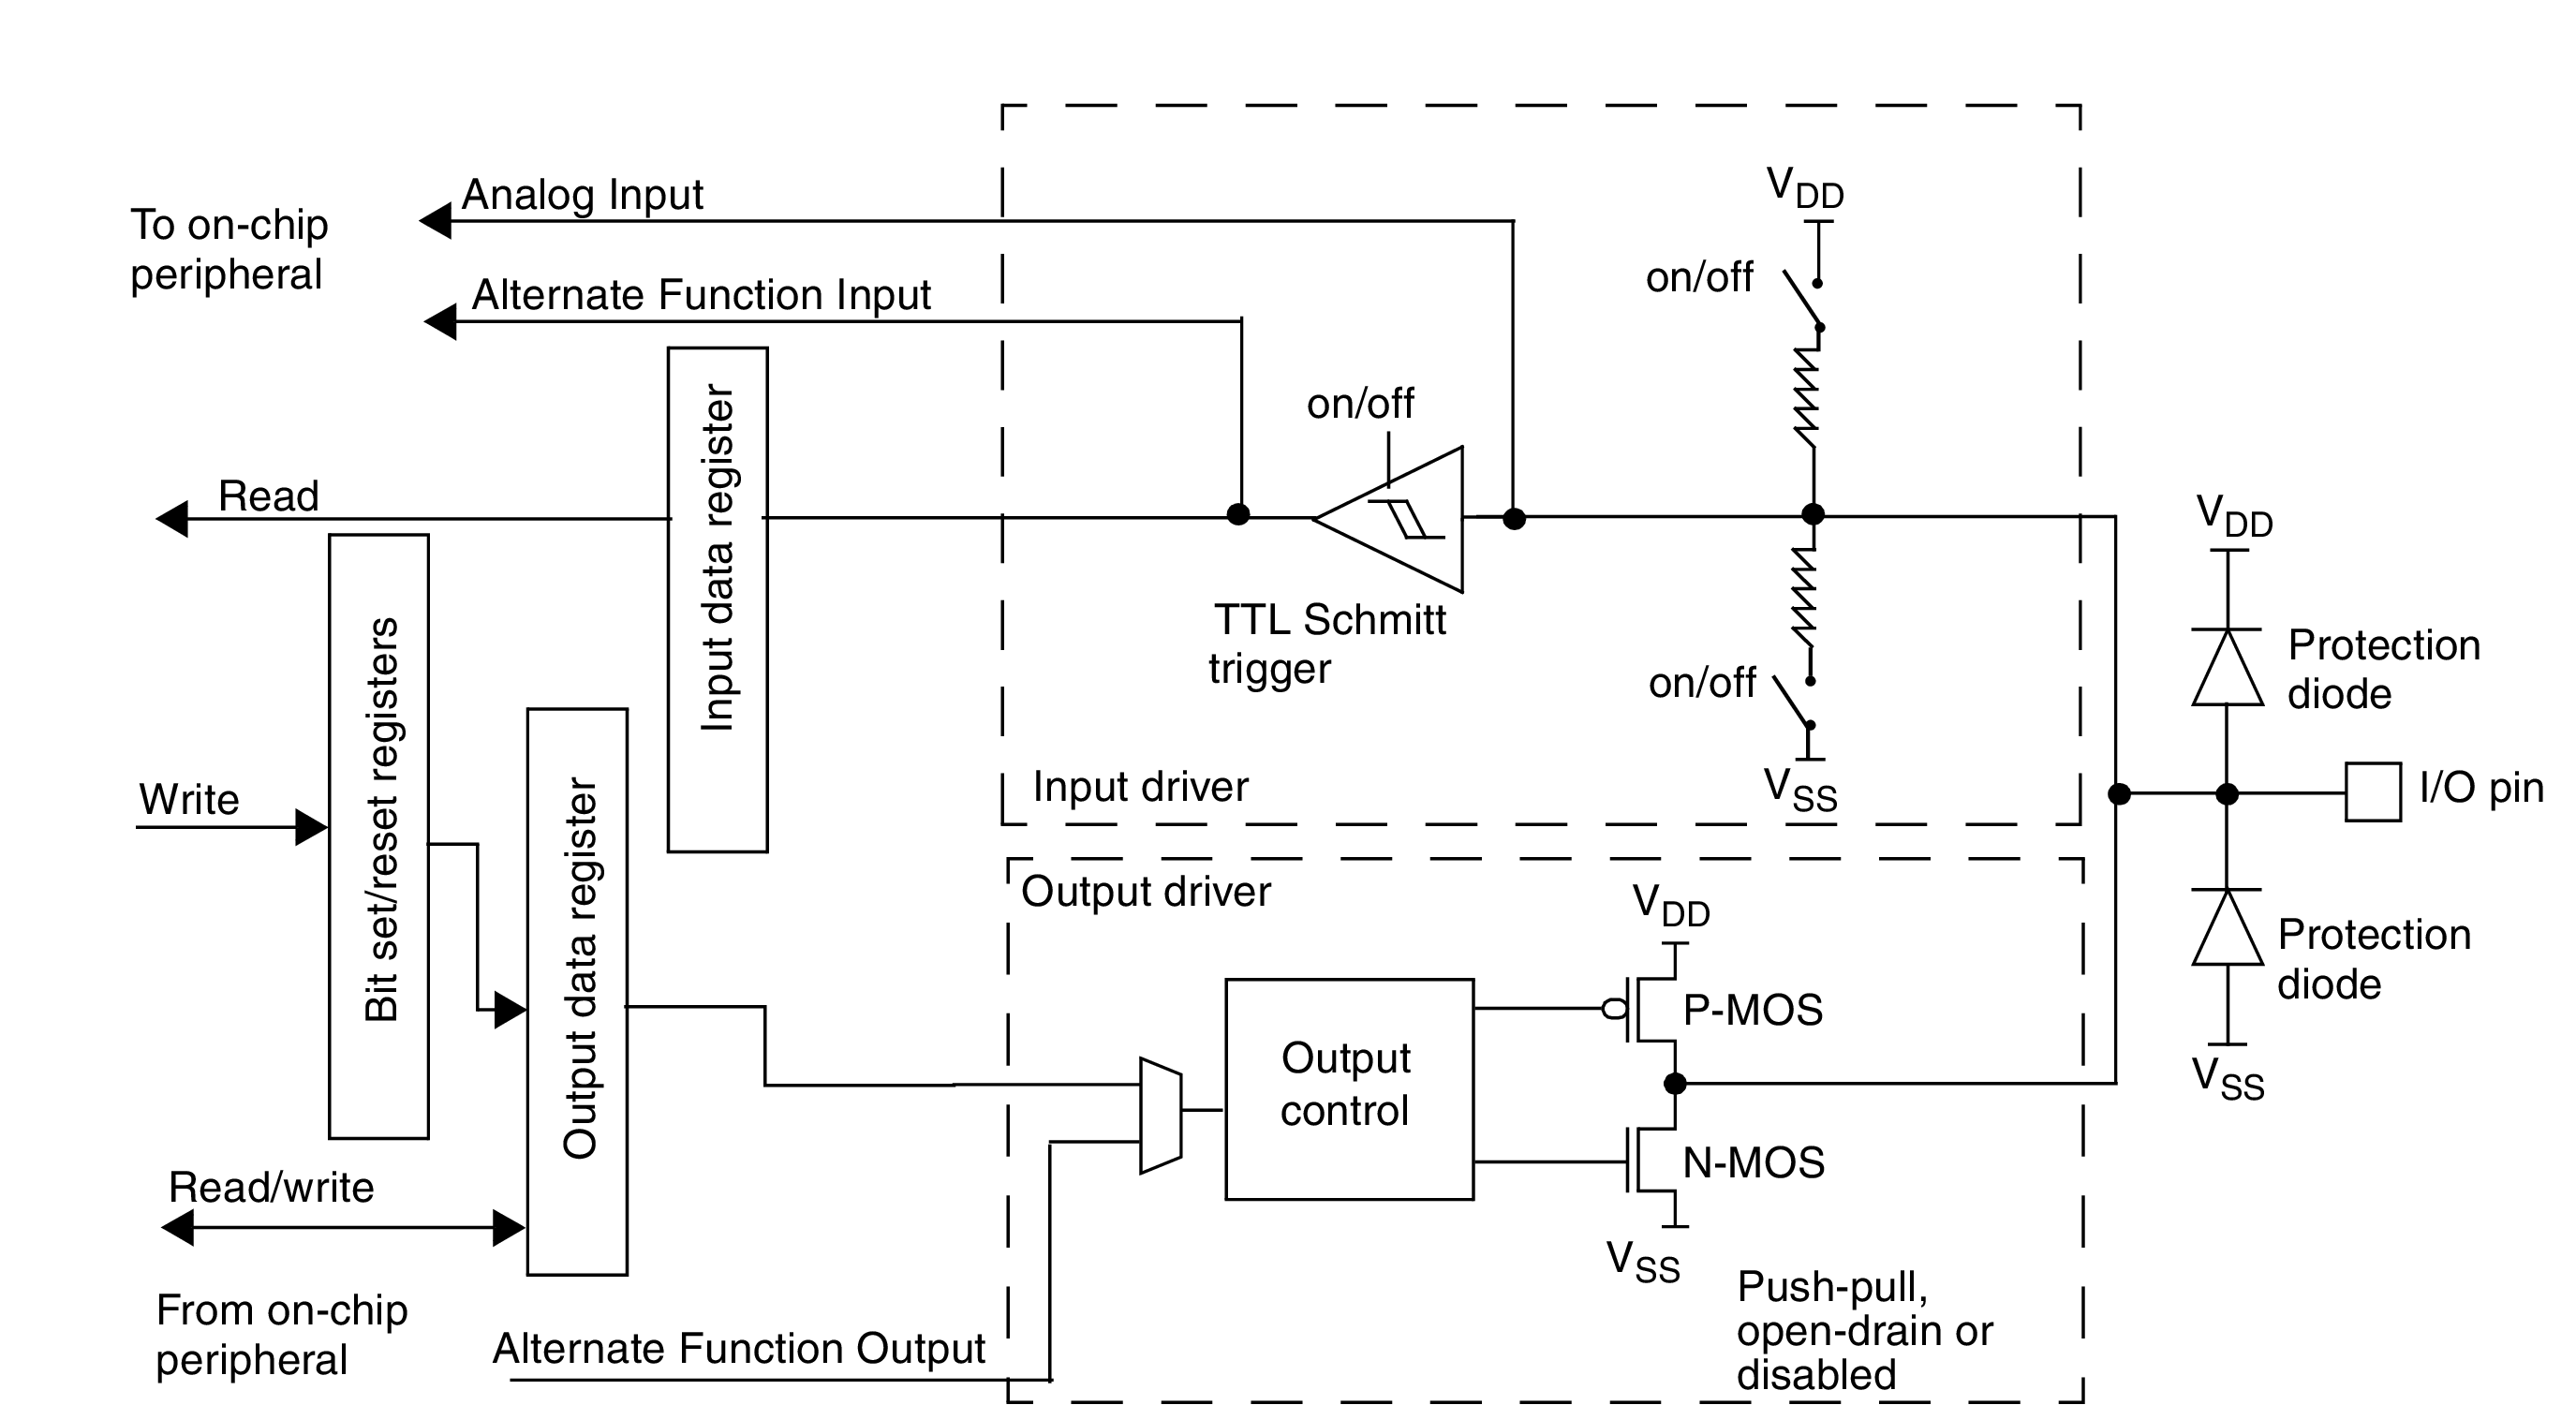
\includegraphics[width=\textwidth]{./img/ioport.png}\caption{STM32 IO Driver System}\label{stm32iodriver}\end{figure}

\subsection{中断控制器配置}

STM32的中断控制是通过NVIC进行集中管理的。在NVIC中,不同中断的优先级可以被自定义,这是通过对多个以\lstinline{NVIC_}开头的寄存器进行写入实现的。为了启用一个中断,程序需要调用的函数是\lstinline{NVIC_Init},其中包括了优先级和启用状态。CMSIS在底层对\lstinline{NVIC_IPRx}进行配置以设定优先级,并对\lstinline{NVIC_ISERx/ICERx}进行配置,以启用或禁用某些中断。通过手动置位\lstinline{NVIC_ISPRx/ICPRx},可以人为的触发或解触发中断。这样,完成了中断的初始化配置过程。

NVIC接受到中断源对应的信号之后,首先通过读取寄存器,判断是否应该对这个中断作出响应。如果是,就按照预订程序,查找中断向量表,其默认地址位于ROM头部(0x20000000)开始的一片区域中\footnote{上次实验中,就手工设定过中断向量表。这次我们让CMSIS帮忙建立。}。之后,根据中断向量表,跳转到对应的子处理程序。子处理程序应该通过检查\lstinline{NVIC_IABRx}确定状态,并在合适的时机置位\lstinline{NVIC_ICPRx},让硬件清除标志位。

在CMSIS中,编写中断处理程序很简单,只要建立对应的函数就好了。如对TIM1的向上溢出中断,对应的函数是\lstinline{TIM1_UP_TIM16_IRQHandler},建立同名的函数,并在函数内用\lstinline{TIM_GetITStatus}确定状态,再用\lstinline{TIM_ClearITPendingBit}清理中断位,表示这个中断已经被处理过,就可以了。

要注意的时,中断服务程序的名称必须正确,最好认真检查,否则可能会触发指令异常错误,让CPU陷入死循环。

\subsection{三种定时器的使用}

这次使用的三种定时器,分别是通用定时器、基本定时器和高级定时器。三者的主要区别是,基本定时器只能向上计数,通用定时器则在其基础上增加了其他两种计数方式(向下和循环),并增加了四个CCP通道,而高级定时器则在其基础上添加了死区等复杂功能。这样,可以用基本定时器进行简单的定时提醒任务,用通用定时器进行简单的PMW发生器,而用高级定时器作为电机驱动桥臂的控制信号源。但我们只需要让LED闪烁,因此用简单的上溢功能就可以了。

定时器和中断是分不开的,一般常常把定时器产生的中断处理掉,或者定时器对应的CCP输出端从内部引出。为了让定时器产生中断,就要先用\lstinline{TIM_ITConfig}打开对应定时器的中断开关,启用对应的项目。比如,上溢中断就是\lstinline{TIM_IT_Update}。之后,要计算定时器的几个装填值,分别是:
\begin{enumerate}
\item 装填值\lstinline{TIM_Prescaler}
\item 计数周期\lstinline{TIM_Period}
\item 计数方式\lstinline{TIM_CounterMode}
\item 分频器设置\lstinline{TIM_ClockDivision}
\end{enumerate}
比如,让小灯以1Hz闪烁,也就是1s触发一次中断,并在中断服务子程序内翻转一次电平。假设SYSCLK为72MHz,那么如果不分频(\lstinline{ClockDivision=0}),就把计数周期设为2KHz,那么\lstinline{TIM_Prescaler}就应该是$$72Mhz / 2kHz = 36k = 36000$$。而要1s触发一次,那么计数周期应该是$$ 2kHz / 1s - 1 = 2000 - 1 = 1999$$,计数方式向上,也就是由0计数到1999。

\subsection{SysTick的重定义}

为了让SysTick能够正确处理,我们需要覆写CMSIS中关于SysTick的处理函数,即\lstinline{SysTick_Handler()}。为了让其闪烁,可以在其中加入一个简单的计数器,达到250即翻转。此外,为了让SysTick能够准确的在每一ms触发一次,还要用\lstinline{SysTick_Config}重新设定SysTick。

\section{程序分析}

程序主文件如清单\ref{mainc}所示,头文件为清单\ref{mainh}所示。这里对代码分片进行大致讲解。

主文件第七行定义了专门用来翻转LED状态的宏blink,第9行开始的主程序调用了初始化函数之后,就进入了死循环。从17行开始,是四个中断服务函数,分别对应着定时器TIM2、TIM0、SysTick和定时器TIM7,LED是从1$\sim$4。启动设备后,1$\sim$4号LED灯分别以2Hz、4Hz、1Hz、8Hz的频率闪烁。

48行开始,就是初始化函数。69$\sim$78行首先打开了GPIO端口,并封锁输出,防止误动作。四个LED是分别链接到E7$\sim$E10上的,推挽输出,50Mhz。之后配置定时器2,计数器触发值36000,溢出界限1000,开中断,从而让TIM2对应的中断每500ms触发一次。TIM0其他参数类似,但是将重复计数器置位1,只有在溢出一次之后再次溢出才会触发中断,也就是触发时间为TIM2的两倍,每1000ms触发一次;TIM7配置同理,但将上界改为250,每125ms中断一次。此外141行还设定了SysTick,重新设定了SysTick的触发值,确定每1ms触发一次。其他代码则是对NVIC的控制,打开了TIM1、2和7的中断。

\section{程序代码}

\begin{lstlisting}[caption={Main file},label={mainc}]
#include "stm32f10x.h"
#include "init_config.h"

// Initilization code
void DeviceInit(void);

#define blink(group, pin)   do{if (GPIO_ReadOutputDataBit((group), (pin)))	GPIO_ResetBits((group), (pin)); else	GPIO_SetBits((group), (pin));}while(0);

int main(void){
	
	DeviceInit();
	
	while(1);
	return 0;
}

void TIM2_IRQHandler(void){//2Hz
	if (TIM_GetITStatus(TIM2, TIM_IT_Update)!=RESET){
		TIM_ClearITPendingBit(TIM2, TIM_FLAG_Update);
		blink(LED_GROUP[0], LED_PIN[0]);
	}
}

void TIM1_UP_TIM16_IRQHandler(void){//1Hz
	if (TIM_GetITStatus(TIM1, TIM_IT_Update)!=RESET){
		TIM_ClearITPendingBit(TIM1, TIM_FLAG_Update);
		blink(LED_GROUP[1], LED_PIN[1]);
	}
}

void SysTick_Handler(void){
	static int systick = 0 ;
	if (systick==250){//4Hz
		blink(LED_GROUP[2], LED_PIN[2]);
		systick=0;
	}else
	systick++;
}

void TIM7_IRQHandler(void){//8Hz
	if (TIM_GetITStatus(TIM7, TIM_IT_Update)!=RESET){
		TIM_ClearITPendingBit(TIM7, TIM_FLAG_Update);
		blink(LED_GROUP[3], LED_PIN[3]);
	}
}


void DeviceInit(void){
	int i = 0;
	GPIO_InitTypeDef gpio_initval;
	NVIC_InitTypeDef nvic_initval;
	TIM_TimeBaseInitTypeDef tim_tb_initval;
	
	
	
	// System clock init
	//SystemInit();
	
	/*
	 * GPIO Initalization
	 *
	 * Since we're using LEDs as a sign of timer's action,
	 * we need to configure some IO ports. LEDs' negative
	 * should be connected to ports defined in init_config.h, 
	 * and 3.3V is connected via a 1K res to positive.
	*/

	//Connect GPIO clock to device clock bus
	RCC_APB2PeriphClockCmd(RCC_APB2Periph_GPIOE, ENABLE);
	for ( i = 0 ; i < LED_numbers; i++ ){
		//Config ports
		gpio_initval.GPIO_Pin = LED_PIN[i];
		gpio_initval.GPIO_Mode = LED_MODE[i];
		gpio_initval.GPIO_Speed = LED_SPEED[i];
		GPIO_Init(LED_GROUP[i], &gpio_initval);
		//Comment following line if you want to turn on LED
		GPIO_SetBits(LED_GROUP[i], LED_PIN[i]);
	}
	
	/*
	 * Timer Initalization
	 *
	 * 
	 */
	//configure TIM2
	RCC_APB1PeriphClockCmd(RCC_APB1Periph_TIM2, ENABLE);  //Connect TIM2 clock to device clock bus
	TIM_DeInit(TIM2);	 //reset to default configure
	//now tim2 clock is 2*(APB1->PCLK1->HCLK/2->SYSCLK/2->36Mhz) = 72Mhz
	tim_tb_initval.TIM_Prescaler = 36000; //72Mhz / 36000 = 2kHz
	tim_tb_initval.TIM_ClockDivision = TIM_CKD_DIV1;	//enable scaler
	tim_tb_initval.TIM_CounterMode = TIM_CounterMode_Up;	//count up
	tim_tb_initval.TIM_Period =  1000;	  	//2khz/1000 = 2hz
	TIM_TimeBaseInit(TIM2, &tim_tb_initval);	//apply settings
	TIM_ClearFlag(TIM2, TIM_FLAG_Update);		//clear flag
	TIM_ITConfig(TIM2, TIM_IT_Update, ENABLE);	//enable interruption
	TIM_Cmd(TIM2, ENABLE);	//enable Timer2
	
	//configure TIM0
	RCC_APB2PeriphClockCmd(RCC_APB2Periph_TIM1, ENABLE);  //Connect TIM1 clock to device clock bus
	TIM_DeInit(TIM1);	//config reset
	tim_tb_initval.TIM_Period = 36000;	//2khz
	tim_tb_initval.TIM_Prescaler = 1000;	//0.5s
	tim_tb_initval.TIM_RepetitionCounter = 1;	//0.5*(0+1)=1s ==> 1hz
	TIM_TimeBaseInit(TIM1, &tim_tb_initval);
	TIM_ClearFlag(TIM1, TIM_FLAG_Update);
	TIM_ITConfig(TIM1, TIM_IT_Update, ENABLE);
	TIM_Cmd(TIM1, ENABLE);	//enable Timer1
	
	//configure TIM7
	RCC_APB1PeriphClockCmd(RCC_APB1Periph_TIM7, ENABLE);  //Connect TIM7 clock to device clock bus
	TIM_DeInit(TIM7);	//config reset
	tim_tb_initval.TIM_Period = 36000;	//2khz
	tim_tb_initval.TIM_Prescaler = 250;	//8hz
	TIM_TimeBaseInit(TIM7, &tim_tb_initval);
	TIM_ClearFlag(TIM7, TIM_FLAG_Update);
	TIM_ITConfig(TIM7, TIM_IT_Update, ENABLE);
	TIM_Cmd(TIM7, ENABLE);	//enable Timer1
	
	/*
	 * NVIC Initalization
	 *
	 * Since timers will trigger some interruptions, we need
	 * to set up the NVICs now. Priorities and some other
	 * values are configured here.
	 */
	//configure TIM2 (General-purpose timers) NVIC
	nvic_initval.NVIC_IRQChannel = TIM2_IRQn;
	nvic_initval.NVIC_IRQChannelCmd = ENABLE;
	nvic_initval.NVIC_IRQChannelSubPriority = 1;
	nvic_initval.NVIC_IRQChannelPreemptionPriority = 0;
	NVIC_Init(&nvic_initval);
	
	//configure TIM0 (Advanced timer) NVIC
	nvic_initval.NVIC_IRQChannel = TIM1_UP_IRQn;
	nvic_initval.NVIC_IRQChannelCmd = ENABLE;
	nvic_initval.NVIC_IRQChannelSubPriority = 2;
	nvic_initval.NVIC_IRQChannelPreemptionPriority = 0;
	NVIC_Init(&nvic_initval);
	
	//configure SYSTick interruption
	SysTick_Config(SystemCoreClock/1000);
	
	//configure TIM7 (Basic timer) NVIC
	nvic_initval.NVIC_IRQChannel = TIM7_IRQn;
	nvic_initval.NVIC_IRQChannelCmd = ENABLE;
	nvic_initval.NVIC_IRQChannelSubPriority = 2;
	nvic_initval.NVIC_IRQChannelPreemptionPriority = 0;
	NVIC_Init(&nvic_initval);
	return;
}
\end{lstlisting}

\begin{lstlisting}[caption={Header file},label={mainh}]
#ifndef __INIT_CONFIG_H__
#define __INIT_CONFIG_H__

#include "stm32f10x.h"

#define LED_numbers 4
//config output (pp-out)
GPIOMode_TypeDef LED_MODE[LED_numbers] = {GPIO_Mode_Out_PP,GPIO_Mode_Out_PP,
	GPIO_Mode_Out_PP,GPIO_Mode_Out_PP};
//clock speed 50m
GPIOSpeed_TypeDef LED_SPEED[LED_numbers] = {GPIO_Speed_50MHz,GPIO_Speed_50MHz,
	GPIO_Speed_50MHz,GPIO_Speed_50MHz};
//ports e7~e10
uint16_t LED_PIN[LED_numbers] = {GPIO_Pin_7, GPIO_Pin_8, GPIO_Pin_9, GPIO_Pin_10};
GPIO_TypeDef* LED_GROUP[LED_numbers] = {GPIOE,GPIOE,GPIOE,GPIOE};

#endif
\end{lstlisting}
\end{document}
